\section{PCA}

\textbf{PCA} uses an orthogonal transformation (vectors multiplied are 0) to
convert a dataset with maybe correlated datas into a dataset withou
correlations.

Rapidminer has a tool applying the PCA algorithm on given data. Output are the
new attributes, which are a combination of the old ones. 

\subsection{Rapidminer Process}
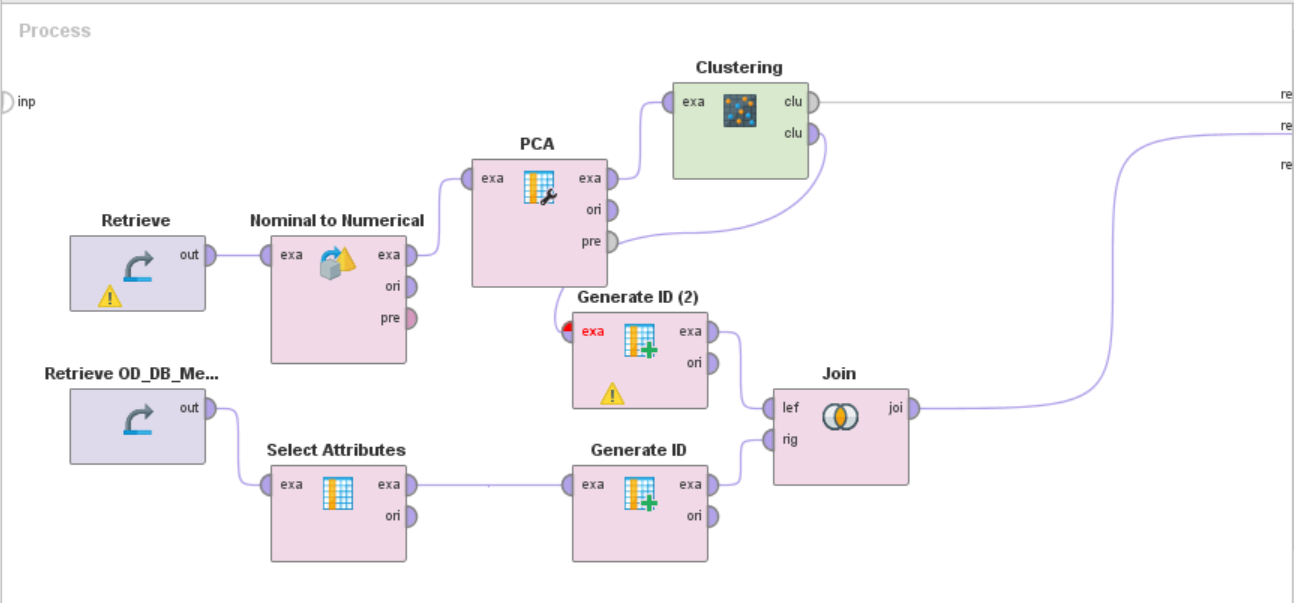
\includegraphics[width=0.9\textwidth]{PCAClustering}

The Process does the following steps:
\begin{description}
	\item[Retrieve] This Block gives the data in the process. For the comparison at the end we also retrieve the original data.
	\item[Nominal to Numerical] This changes the nominal data to numerical data, so that we can apply PCA in the next step
	\item[PCA] Here we apply the PCA reduction to the data with a variance threshold $0.95$
	\item[Clustering] Here the number of Clusters has to be fixed. We decided, that 10 runs should be enough. We can choose between differen measure types and tried mixed euclidean and squared euclidean distance
	\item[Generate ID] Is just needed to join the datasets 
	\item[Select Attribute] Here we just pick the Strata data for comparing with the clustering
	\item[Join] For comparing the Clustering and the Strata we join the two filtered data sets at the ID
\end{description}

This is the basis for all datasets.

\subsection{Applying on original data}
Applying the PCA module on the original data without EST and a variance
threshold of 0.95 we get two Attributes, so we can assume, that the data is strongly connected. As expected the computating time decreases a lot. 

For a clustering of 6 clusters we get a distribution that is complete different from the original distribution \ref{fig:OrgDist}. 
\begin{figure}
\centering
\begin{subfigure}{.5\textwidth}
  \centering
  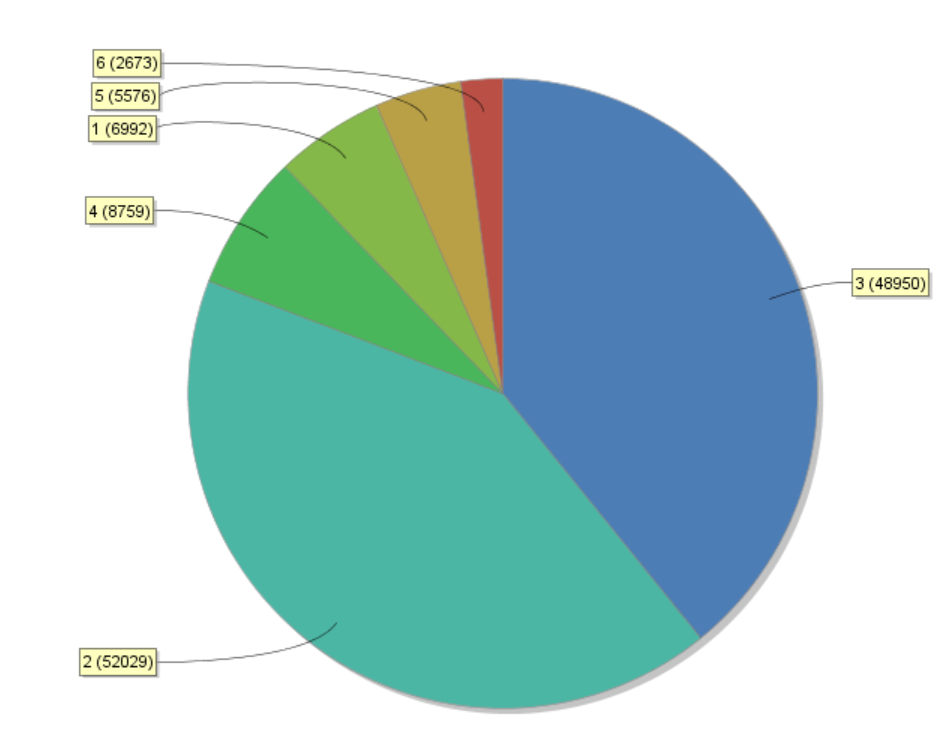
\includegraphics[width=.4\linewidth]{ClusterOrigRapidStrata.PNG}
  \caption{Strata}
  \label{fig:OrgSt}
\end{subfigure}%
\begin{subfigure}{.5\textwidth}
  \centering
  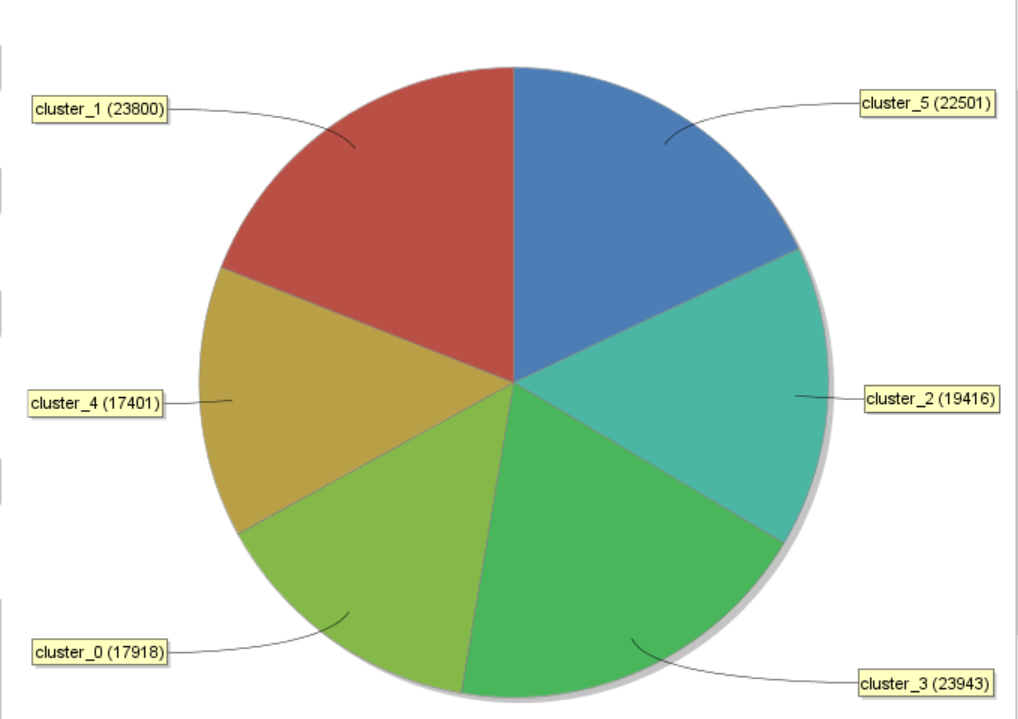
\includegraphics[width=.4\linewidth]{ClusterOrigRapidCluster.PNG}
  \caption{Cluster}
  \label{fig:OrgCl}
\end{subfigure}
\caption{Distribution of original data}
\label{fig:OrgDist}
\end{figure}
